The Smart Cart shall consist of four major layers, namely the power supply layer, imaging layer, crab drive layer and cart hardware layer. The power supply layer shall comprise mainly the power supply subsystem. The image capturing layer shall include the camera subsystem. The cart hardware layer shall contain the switch subsystem and the wheels. Lastly, the cart navigation layer shall include the drive subsystem.

\begin{figure}[h!]
	\centering
 	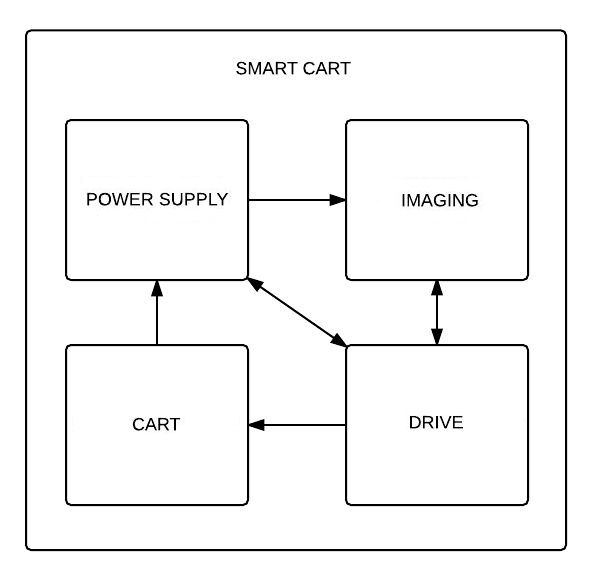
\includegraphics[width=0.60\textwidth]{images/system_overview}
 \caption{A simple architectural layer diagram}
\end{figure}


\subsection{Power Supply Layer Description}
The power supply layer shall include the main power source both to the cart and to the sockets to which external devices shall be plugged. This subsystem shall contain a 12V deep cycle battery, a 2 to 3V regulator, a 5V voltage converter, and a recharge switch. The voltage regulator shall regulate the power made available for charging devices. The voltage converter shall convert 12V to a stable 5V to power the Smart Cart. Lastly, the recharge switch shall be used to protect electronics while the battery charges.

\subsection{Cart Layer Description}
The cart layer shall include a manual switch, a killswitch, and the wheels. The manual switch that shall be used to selectively pause the system and allow the user to use the cart in manual mode. The killswitch shall be used to turn off the Smart Cart system in the event of an emergency. Lastly, the wheels shall move the cart.

\subsection{Crab Drive Layer Description}
The crab drive layer shall include a main motor, drive system interface with the processor, the main motor, and four individual wheel motors. This layer will control and process the navigation of the cart. The main motor processes and control the chain/belt system which coordinates the individual wheel motors.

\subsection{Imaging and Navigation Description}
The imaging layer shall include sensors and the camera interface. This layer will get visual data for recognising and following the user and detecting obstacles.
